\def\year{2019}\relax
%File: formatting-instruction.tex
\documentclass[letterpaper]{article} %DO NOT CHANGE THIS

%%proofreading
%\usepackage{setspace}
%\doublespacing

\usepackage{multirow}
\usepackage{amsmath}
\usepackage{amsfonts}
\usepackage{booktabs}
\usepackage{array}
\newcommand{\Ep}{\mathbb{E}}
\newcommand{\Real}{\mathcal{R}}
\newcommand{\Rating}{\mathbf{X}}
\newcommand{\Loss}{\mathcal{L}}
\usepackage{aaai19}  %Required
\usepackage{times}  %Required
\usepackage{helvet}  %Required
\usepackage{courier}  %Required
\usepackage{url}  %Required
\usepackage{graphicx}  %Required
\frenchspacing  %Required
\setlength{\pdfpagewidth}{8.5in}  %Required
\setlength{\pdfpageheight}{11in}  %Required
%PDF Info Is Required:
  \pdfinfo{
/Title ()
/Author (AAAI Press Staff)}
\setcounter{secnumdepth}{0}  
 \begin{document}
% The file aaai.sty is the style file for AAAI Press 
% proceedings, working notes, and technical reports.
%
\title{Non-Compensatory Psychological Models for Recommender Systems}
\author{ID: 335
}
\maketitle
\begin{abstract}
The study of consumer psychology reveals two categories of consumption decision procedures: compensatory rules and non-compensatory rules. Existing recommendation models which are based on latent factor models assume the consumers follow the compensatory rules, i.e. the consumer evaluates an item over multiple aspects and computes a weighted or/and summated score which is further used to derive the rating or ranking of an item. However, it has been shown in the literature of consumer behavior that, consumers adopt non-compensatory rules more often than compensatory rules. Our main contribution in this paper is to study the unexplored area of utilizing non-compensatory rules in recommendation models. 

Our general assumptions are (1) there are $K$ universal hidden aspects. In each evaluation session, only one aspect is chosen as the prominent aspect according to user preference. (2) Evaluations over prominent and non-prominent aspects are non-compensatory. Evaluation is mainly based on item performance on the prominent aspect. For non-prominent aspects the user sets a minimal acceptable threshold. We give a conceptual model for these general assumptions and show how this model can be realized to a wide range of existing recommender systems, including  point-wise rating prediction models and pair-wise ranking prediction models.  We experimentally show that adopting non-compensatory rules constantly improve recommendation performance of different existing models on a variety of real-world data sets.
\end{abstract}



\section{Introduction}\label{sec:introduction}
The majority of state-of-the-art recommendation models are based on latent factor models. Generally, latent factor models transform both user preferences and item features into the same hidden feature spaces with $K$ aspects. To recover the observations (i.e. ratings or rankings) in any recommender system, they adopt the inner products of the user preferences and the item features. There are fruitful successful applications of latent factor models in  rating predictions~\cite{Koren2009Matrix,Koren2010Factor,Lee2014Local} and ranking reconstructions~\cite{Rendle2009BPR,Steck2015Gaussian,Zhao2018Factored,Shi2010List}.   

From the perspective of consumer decision making, all existing latent factor models fall into the category of \emph{compensatory rules}. Under compensatory rules a consumer will evaluate an item over all aspects, thus a good performance on one aspect of an item compensates for poor performances on other aspects. For example, Alice wants to buy a cellphone and she is concerned about three relevant aspects: battery life, price and storage space. A compensatory rule to evaluate a cellphone is to score its performance on each aspect separately and compute a weighted summation over all aspects.


However, in the study of human choice behavior, it is well regarded that consumers more frequently make consumption related choices based on \emph{non-compensatory rules}~\cite{Engel1986Consumer}. For example, ~\cite{Hauser2009Non} reviews $132$ empirical surveys in literature and  concludes that more than $70\%$ of consumers adopt non-compensatory rules when buying air-conditioners, automobiles, computers, cameras and so on. 

Non-compensatory rules do not allow the shortcomings of a product to be balanced out by its attractive features. The literature has proposed different non-compensatory rules, among which  \emph{lexicographic rule} and \emph{conjunctive rule} are the most common. For example, in a survey interviewing consumption decisions about beer brands and fast-food outlets~\cite{Laroche2003Which}, conjunctive rule has a success rate of $62.0\%$ in predicting brand consideration and lexicographic rule has a success rate of $34.6\%$ which is the second highest non-compensatory rule. We next illustrate  \emph{lexicographic rule} and \emph{conjunctive rule}  by the cellphone example in Table~\ref{tab:example}. 

\textbf{Example.} Lexicographic rule assumes that aspects of products can be ordered in terms of importance and alternative brands are evaluated sequentially from most prominent to least prominent aspects.  If Alice's priority is long-lasting battery, then she will adopt lexicographic rule to rank phones first based on battery life. In this case Honor and iPhone will be ranked higher than Galaxy. The other benefits offered by Galaxy  do not outweigh her desire for a long-life battery. Conjunctive rule establishes a minimally acceptable threshold for each aspect. Evaluation is made on the basis of whether or not the products satisfy the threshold. If Alice wants the phone to be cheap and with plenty of storage space, then she will adopt conjunctive rule to set thresholds (e.g. $600\$$ and $64GB$ on the corresponding aspects). In this case, iPhone fails to meet the cut-off point, thus it will not outrank Honor. In either case, adopting a compensatory rule based recommendation model is problematic. 

\begin{table}[htp]\label{tab:rules}
\caption{The cellphone example to illustrate non-compensatory rules.}
\begin{center}
\begin{tabular}{|c|c|c|c|}
\hline
Item & Prominent aspect & \multicolumn{2}{|c|}{Non-prominent aspects}\\\hline
& Battery life &  Price & Memory \\\hline
iPhone SE &  13 hours & 700$\$$ & 64GB  \\\hline
Galaxy S8 & 9 hours& 500$\$$  & 128GB \\\hline
Honor 10 & 24 hours& 589$\$$ & 128GB \\\hline
\end{tabular}
\end{center}
\label{tab:example}
\end{table}%

Current computer support for non-compensatory rules is to manually control the rules in decision support systems~\cite{Lee2009Transforming}, e.g. consumers are asked to specify the threshold for an aspect of interest. Such manual approaches are labor costly and difficult to set up and maintain. On the contrary, learning models such as latent factor models~\cite{Koren2009Matrix} have the advantage of scalability, simplicity and flexibility. Unfortunately, to the best of our knowledge, no previous effort has been devoted to building learning to recommend models based on non-compensatory rules. 

Our goal in this paper is to study this unexplored area of how learning models can benefit from non-compensatory rules. Two challenges need to be addressed. (1) How to embed symbolic non-compensatory rules in a data-driven learning framework? (2) How to present a general framework based on non-compensatory rules in a manner that complies with a variety of existing recommendation models, including rating prediction and ranking aware models?  

Our primary contribution is to give a conceptual model of how users adopt non-compensatory rules in recommender systems. Our assumptions are based on the lexicographic and conjunction rules. We assume that, (1) there are $K-$ hidden aspects which  user preferences and item features are transformed into, (2) in each evaluation session, the user picks a prominent aspect according to his/her preference, (3) the user adopts different evaluation strategies on prominent and non-prominent aspects. The evaluation is mainly based on item performance on the prominent aspect. The evaluation is less influenced by item performance with respect to user-defined minimal acceptance values on non-prominent aspects.

Our second contribution is to realize the conceptual model in a wide range of recommendation frameworks, including point-wise rating prediction models such as the conventional Matrix Factorization (MF~\cite{Koren2009Matrix}), Matrix Factorization with neighborhood collaborative filtering (AMF~\cite{Koren2008Factorization}), and local low-rank matrix approximation (LLORMA~\cite{Lee2013Local}), and pairwise ranking reconstruction models such as the Bradley-Terry model (BT~\cite{Hu2016Improved}) and Thurstone model (BPR~\cite{Rendle2009BPR}). 

We conduct comprehensive experiments on a variety of real world data sets. We experimentally show that \emph{ the proposed non-compensatory framework universally improves recommendation performances of different existing models}. 

The paper is organized as follows. We start with surveying the most commonly adopted latent factor models. We show that previous research work is based on compensatory rules. Next, we present a conceptual model based on non-compensatory rules and realize it in different existing models. Then, we experimentally show that the non-compensatory modifications outperform the original versions of existing models on a variety of real-world data sets. Finally we conclude our work.

\section{Compensatory Recommendation Models}\label{sec:previousmodel}
In this section, we show that existing latent factor models can be categorized based on the forms of rating prediction formulas and loss functions. Table~\ref{tab:summary} summarizes typical related work. We restrict our discussions to latent factor models, i.e. models where a universe of $K$ factors is used to project  user preferences and item features. Hereafter, unless stated otherwise, we use lower-case letters for indices, upper-case letters for universal constants, lower-case bold-face letters for vectors and upper-case bold-face letters for matrices. Specifically, $\mathbf{X}\in \Real^{M\times N}$ denotes the rating matrix, $\hat{\mathbf{X}}\in \Real^{M\times N}$ denotes the predicted rating matrix,  $\mathbf{p},\mathbf{q}\in \Real^K$ denotes the item features, which are rows of item space $\mathbf{V}\in \Real^{N\times K}$, $\mathbf{u}\in \Real^K$ denotes the user preferences, which is a row of the user space $\mathbf{U}\in \Real^{M\times K}$.  $\mathbf{U},\mathbf{V}$ are components of the model parameters $\Theta=\{\mathbf{U},\mathbf{V} \}$.

\begin{table*}[htp]
\tiny
\caption{Existing latent factor models in literature can be classified based on the loss functions and rating prediction formulas.}
\begin{center}
\begin{tabular}{|c|c|c|c|}
\hline
\multirow{2}{*}{Loss Function} &\multicolumn{3} {|c|}{Rating Prediction Formula}\\\cline{2-4}
& Matrix Factorization & Neighborhood Factorization & Local Low-rank Factorization \\\hline
Point-wise Square Loss & MF ~\cite{Koren2009Matrix} & AMF ~\cite{Koren2008Factorization} & LLORMA~\cite{Lee2013Local}\\\hline
Pair-wise Thurstone Ranking & BPR~\cite{Rendle2009BPR} & FSBPR~\cite{Zhao2018Factored} & LCR~\cite{Lee2014Local} \\\hline
Pair-wise BT Ranking & BT~\cite{Hu2016Improved} & - & -  \\\hline
\end{tabular}
\end{center}
\label{tab:summary}
\end{table*}%

\subsection{Rating Prediction Formulas}
One goal of recommendation research is to recover the rating matrix $\Rating$, by minimizing a rating aware loss function $\Loss(\Theta)$, which is usually defined as the regularized square loss between the predicted rating $\hat{\Rating}_{u,q}$ and the observed rating $\hat{\Rating}_{u,q}$ for each user $u$ who has rated item $q$. 
\begin{equation}\label{equ:ratingloss}
\Loss(\Theta)=\sum_{u,q}(\Rating_{u,q}-\hat\Rating_{u,q})^2 + \lambda (\|\mathbf{U}\|+\|\mathbf{V}\|)
\end{equation}
We list some of the most successful rating prediction formulas for $\hat{\Rating}$.

\textbf{Matrix Factorization.} In conventional Matrix Factorization (MF)~\cite{Koren2009Matrix}, the predicted rating can be computed as an inner product of user preferences and item features as follows.
\begin{equation}\label{equ:MF}
 \hat{\mathbf{X}}_{u,q}=\sum_{k=1}^{K} \mathbf{q}_k \mathbf{u}_k
\end{equation}

For simplicity we ignore the user specific or item specific bias~\cite{Koren2009Matrix}. A massive amount of techniques have been proposed based on Equ.~\ref{equ:MF}. Most of them modified the loss function ,e.g. by incorporating prior distributions over $\mathbf{p},\mathbf{u}$~\cite{salakhutdinov2008probabilistic}, adding priors over unknown values~\cite{Devooght2015Dynamic}, weighing different samples~\cite{Pil'aszy2010Fast} and so on.  

\textbf{Neighborhood Factorization}. In traditional memory based collaborative filtering strategies, neighborhood information has been proved to be useful. It is possible  to incorporate such neighborhood information in latent factor models. Instead of directly modeling user preferences $\mathbf{u}$, each user is represented by items that he/she gives explicit or implicit feedback. For example, if we consider explicit feedback only, then each item is associated with two types of vectors $\mathbf{p},\mathbf{q}$, the rating prediction formula of Asymmetric Matrix Factorization (AMF) in ~\cite{Koren2008Factorization} is stated as follows.  
 \begin{equation}\label{equ:AMF}
\hat{\Rating}_{u,q}=\sum_{k=1}^{K} \mathbf{q}_{k} (\sum_{p \in R(u)} \mathbf{p}_k/\sqrt{|R(u)|} ),
\end{equation}
where  $R(u)$ is the set of rated items for $u$. AMF has been extended to SVD++~\cite{Koren2008Factorization} with implicit feedback. 

\textbf{Local Low-Rank Matrix Approximation.} The third type of rating prediction formula is  Local Low-Rank Matrix Approximation (LLORMA)~\cite{Lee2013Local}. The intuition is that the entire rating matrix $\Rating$ is not low-rank but a sub-matrix restricted to a neighborhood of similar users and items is low-rank.  Therefore, the predicted rating is aggregated over $S$ sub-matrices  as follows:
\begin{equation}\label{equ:LLORMA}
\hat{\Rating}_{u,q} = \sum_{t=1}^{S} \sum_k \mathbf{u}_{t, k} \frac{K((\mathbf{u}_t,\mathbf{i}_t),(\mathbf{u},\mathbf{q}))}{\sum_{s=1}^{S} K((\mathbf{u}_s,\mathbf{i}_s),(\mathbf{u},\mathbf{q}))} \mathbf{q}_{t,k},
\end{equation}
where $\mathbf{u}_t, \mathbf{q}_t$ are the factorized user preferences and item features in the $t-$th sub-matrix,  $\mathbf{i}_s,\mathbf{i}_t$ are anchor points in the corresponding matrix to locate a neighborhood for low-rank decomposition, $K(\cdot)$ is a smoothing kernel. 


\subsection{Ranking Models}
Another goal of recommendation research is to reveal the observed rankings. We here consider pair-wise rankings $p\succ_u q$, where user $u$ prefers item $p$ over $q$. The pair-wise rankings can be generated from pre-processing  the ratings, i.e. $\Rating_{u,p}> \mu, \Rating_{u,q}<\mu$~\cite{Hu2017Decoupled}, or from explicit and implicit feedback, i.e. $\Rating_{u,p}\neq 0$ and $ \Rating_{u,q}$ doesn't exist~\cite{Rendle2009BPR}. 

A large body of previous research has been presented by employing a ranking aware loss function  $\Loss(\Theta)$ on the observed pair-wise rankings. For example, the Bayesian posterior is expressed as:
\begin{equation}
\Loss(\Theta) = \sum_{u}\sum_{p,q} o(p\succ_u q) \log p(p\succ_u q) + \lambda(\|\mathbf{U}\| + \|\mathbf{V}\|),
\end{equation}
where $p(p\succ_u q)$ is the predicted possibility and $o(p\succ_u q)$ is an indicator function of whether or not the ranking is observed. 

To generate the probability of pair-wise rankings $p(p\succ_u q)$,  each user-item combination is associated with a score, i.e. $\hat{\Rating}_{u,p},\hat{\Rating}_{u,q}$.  We list two most commonly adopted ranking models . 


\textbf{Thurstone Model} The most frequently adopted ranking model in recommendation systems is the Thurstone model~\cite{Thurstone1927law} which uses a non-linear transformation of the predicted ratings. 
\begin{equation}
p(p\succ_u q) = \frac{1} {1+\exp[-(\hat{\Rating}_{u,p}-\hat{\Rating}_{u,q})]}
\end{equation}

Thurstone model with standard matrix factorization prediction formula is first presented as BPR~\cite{Rendle2009BPR}, which maximizes the Bayesian posterior with respect to Thurstonian modeling of standard matrix factorization predictions. Abundant research has been carried out to improve BPR-style systems by modifying the sampling methods in optimization, including BTR++~\cite{Lerche2014Using}, WARP~\cite{Weston2011Wsabie}, DNS~\cite{Zhang2013Optimizing}, RankMBPR~\cite{Yu2016RankMBPR} and so on.

\textbf{Bradley-Terry Model.} Another extensively studied model in learning to rank scenarios is the Bradley-Terry model~\cite{Hunter2004MM}, which generates ranking pairs by a division:
\begin{equation}\label{equ:BT}
p(p\succ_u q) = \frac{\exp{\hat{\Rating}_{u,p}}}{\exp{\hat{\Rating}_{u,p}}+ \exp{\hat{\Rating}_{u,q}}}.
\end{equation}
BT model in~\cite{Hu2016Improved} leverages the MF prediction formula  in $\hat{\Rating}_{u,p}$. 

The list is by no means exclusive. However, we believe that most of existing recommender systems are covered. It is worthy to point out that (1) we do not restrict the form of loss functions. For example, many ranking approaches consider Bayesian maximum posterior, cross entropy and other forms of loss functions. Nevertheless, the core ranking model is either BT or Thurstone. (2) Although we only study pair-wise ranking , the conclusion is insightful for other ranking-aware systems, i.e. point-wise and list-wise approaches. The reason is that, as shown in ~\cite{Steck2015Gaussian},  point-wise and list-wise loss functions can be decomposed to components which are directly based on each score $\hat\Rating_{u,q}$ and components that are not related to $\hat\Rating$. Thus our proposed strategy in the next section is also applicable to point-wise and list-wise ranking models. (3) As the key component $\hat\Rating_{u,q}$ is based on compensatory rules, all existing latent factor models are essentially compensatory. 

\section{Non-Compensatory Recommendation Models}\label{sec:Nmodel}
We begin this section by reviewing the findings in consumer psychology study. We proceed to present a general framework for modeling the psychological assumptions about non-compensatory rules. We show the universality of the proposed framework by realizing it in different rating prediction formulas and ranking models.

We can see that non-compensatory rules differ from compensatory rules in two key points. (1) \textit{Distinguished factors}. In compensatory rules, different factors are essentially equivalent, while in non-compensatory rules factors are not interchangeable. (2) \textit{Distinguished evaluation metrics on each factor}. In compensatory rules, the evaluations on each factor follow the same framework (i.e. a product of user preference and item feature on the specific factor), while in non-compensatory rules, the evaluations on each factor are dissimilar.  

For computational convenience, inspired by the psychological findings, we present the conceptual model in Fig.~\ref{fig:model} based on lexicographic and conjunction rules. We assume that in each evaluation session\footnote{The evaluation session could be either a true user interaction session with multiple actions, or a pseudo session which contains one rating action. The impact of availability of session information is discussed in experiments. }, there is a prominent aspect. The choice of the prominent aspect is dependent on the user preferences. Two types of evaluation strategies are adopted, one for the prominent aspect and the other for other non-prominent aspects. Evaluation on the prominent aspect is enhanced by strength coefficient $\theta$. Evaluations on non-prominent aspects are based on item performance, compared with the user-defined aspect-specific threshold $\mathbf{b}_u$. The overall evaluation, which could be either a rating or a ranking, aggregates over prominent and non-prominent aspects. 

 \begin{figure}[htbp]
\begin{center}
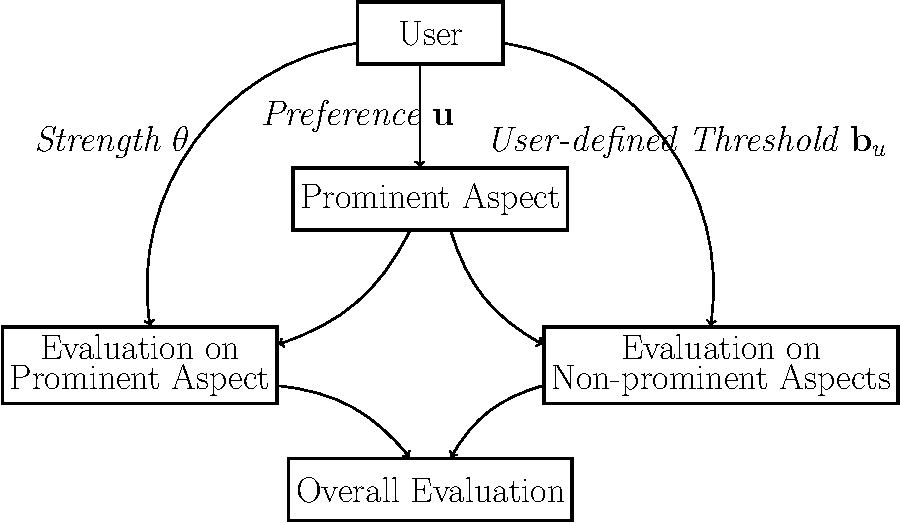
\includegraphics[width=0.4\textwidth]{conceptualmodel.pdf}
\caption{Conceptual model of the user evaluation process}
\label{fig:model}
\end{center}
\end{figure}


\subsection{Non-Compensatory Rating Prediction Formulas}
Given user preference vector $\mathbf{u}$, in each evaluation session, the hidden prominent aspect is sampled by $k\sim \frac{\exp \mathbf{u}_k}{\sum_{k'} \mathbf{u}_{k'}} $. Evaluation on the prominent aspect is magnified by  $\exp \theta$. Evaluation on a non-prominent aspect is denoted as $q_k-\mathbf{b}_{u,k}$. Thus, when the aspect $k$ is chosen, the evaluation of user $u$ on $q$ is $\mathbf{q}_k \exp\theta  + \sum_{k'\neq k} (\mathbf{q}_{k'}-\mathbf{b}_{u,k'})$. The prediction is generated across all possible hidden prominent aspects. This gives us the following non-compensatory versions of rating prediction formulas.

\textbf{Non-compensatory Matrix Factorization: MF-N} 
\begin{equation}\label{equ:MF-N}
 \hat{\mathbf{X}}_{u,q}=\sum_{k=1}^{K} \frac{\exp \mathbf{u}_k}{\sum_{k'} \exp \mathbf{u}_{k'}} [ \mathbf{q}_k  \exp\theta  + \sum_{k'\neq k} (\mathbf{q}_{k'}-\mathbf{b}_{u,k'}) ]
\end{equation}


\textbf{Non-compensatory Neighborhood Factorization: AMF-N} implements a similar scheme by setting $u_k =\sum_{p \in R(u)} \mathbf{p}_k/\sqrt{|R(u)|} $, 
\begin{equation}\label{equ:AMF-N}
 \hat{\mathbf{X}}_{u,q}=\sum_{k=1}^{K} \frac{\exp (\sum_{p \in R(u)} \mathbf{p}_k )}{\sum_{k'} \exp  (\sum_{p \in R(u)} \mathbf{p}_{k'} ) } [  \mathbf{q}_k \exp\theta + \sum_{k'\neq k} (\mathbf{q}_{k'}-\mathbf{b}_{u,k'}) ].
\end{equation}

\textbf{Non-compensatory Local Low Rank Matrix Approximation: LLORMA-N} uses the same decomposition for each sub-matrix.  
\begin{eqnarray}\label{equ:LLORMA-N}
\hat{\Rating}_{u,q} = & \sum_{t=1}^{S} \sum_k  \frac{\exp \mathbf{u}_k}{\sum_{k'} \exp \mathbf{u}_{k'}}  \frac{K((\mathbf{u}_t,\mathbf{i}_t),(\mathbf{u},\mathbf{q}))}{\sum_{s=1}^{S} K((\mathbf{u}_s,\mathbf{i}_s),(\mathbf{u},\mathbf{q}))} \\\nonumber
& [ \mathbf{q}_{t,k} \exp\theta  + \sum_{k'\neq k} (\mathbf{q}_{t,k'}-\mathbf{b}_{u,k'}) ]
\end{eqnarray}

We can see that all these non-compensatory versions are combinations of lexicographic and conjunction rules, where  $\exp\theta \rightarrow \infty$ indicates that the user adopts lexicographical rules only. The threshold for a user on an aspect is static in the sense that $\mathbf{b}_{u,k}$ does not change by the nature of the items.

\subsection{Non-Compensatory Ranking Models}

\textbf{Non-compensatory Thurston Model}. The modification of Thurston model is straightforward, as the ranking probability involves a subtraction component of $\hat\Rating_{u,q}$ which can be replaced by any N-version of rating prediction formulas. Note that the user-defined aspect specific threshold $\mathbf{b}_{u,k}$ cancels between $\hat\Rating_{u,p}$ and $\hat\Rating_{u,q}$.

Inference of Thurston models is also easily extensible. For example, to derive BPR-N, the non-compensatory version of BPR~\cite{Rendle2009BPR}, we alter the stochastic gradient descent (SGD) in inference with $\frac{\partial \Loss}{\partial \Theta}=  \sum_u \sum_{p\succ_u q} \frac{\partial \Loss}{\partial \Delta\hat{\Rating}_{u,p,q} } \frac{\partial \Delta\hat{\Rating}_{u,p,q}  }{\partial \Theta}$, where $\Delta\hat{\Rating}_{u,p,q} =\hat{\Rating}_{u,p}-\hat{\Rating}_{u,q}$. The same procedure applies to modifying FSBPR~\cite{Zhao2018Factored} and LCR~\cite{Lee2014Local}.



\textbf{Non-compensatory Bradley-Terry Model.} Finally we propose BT-N, the non-compensatory version of BT~\cite{Hu2016Improved}. In order to treat prominent and non-prominent aspects differently, we define the probability of any ranking pair $p\succ_u q$ as the product of results by factor-wise comparisons. Intuitively $p$ outranks $q$ suggests that $p$ is significantly better on the prominent aspect, and not too bad on non-prominent aspects. Inspired by a variant of BT model with ties~\cite{Hunter2004MM}, given a hidden prominent aspect $k\sim u_k$ sampled for the evaluation session, we define the factor-wise ranking probability on prominent aspect $k$ as ${\frac{\mathbf{p}_k}{\mathbf{p}_k+\theta \mathbf{q}_k}}$, and ranking probability on non-prominent aspect $k'$ as $ \frac{\theta \mathbf{p}_{k'}}{\mathbf{q}_{k'}+\theta \mathbf{p}_{k'}}$. The overall prediction is aggregated over all possible hidden prominent aspect $k$:
\begin{equation}\label{equ:BT-N}
p(p\succ_u q)  =  \prod_{k=1}^{K} \mathbf{u}_k [ {\frac{\mathbf{p}_k}{\mathbf{p}_k+\theta \mathbf{q}_k}}\prod_{k'\neq k}{ \frac{\theta \mathbf{p}_{k'}}{\mathbf{q}_{k'}+\theta \mathbf{p}_{k'}}}],
\end{equation}
where $\mathbf{u}_k >0, \sum_k \mathbf{u}_k=1,\mathbf{p,q}>\mathbf{0}$ and $\theta>1$.  

BT-N is also a combination of lexicographic rules and conjunction rules. (1) $\theta$ controls the strength of evaluation on the prominent aspect. Consider only the prominent aspect, the evaluation requires $p_{k} > \theta q_{k}, \theta>1$ to generate a positive ranking $p\succ q$. Thus a larger value $\theta$ indicates that the user is more strict on the prominent aspect. When $\theta \rightarrow \infty$, the probability from non-prominent aspects  approaches to one, the users adopt lexicographic rules only. (2) The model sets threshold in a dynamic manner. $p$ is considered to be as good as $q$ on a non-prominent aspect $k'$, as long as $\theta p_{k'} >  q_{k'},\theta>1$.  An interpretation is that the user sets a minimal acceptance threshold for $p_{k'}$ based on the compared alternative $q_{k'}$, where the threshold is $q_{k'}/\theta$.  

To infer the parameters of BT-N, we implement a stochastic expectation maximization (SEM) algorithm. In each E-step, we first draw the value of prominent aspect $k$ for each evaluation session by
 \begin{equation}
 k \sim u_k^{t} \frac{\mathbf{p}_{k}^t} {\mathbf{p}_{k}^t+\theta^t \mathbf{q}_{k}^t} \prod_{k'\neq k}  [\frac{\theta^t \mathbf{p}_{k'}^t} {\mathbf{q}_{k'}^t + \theta^t \mathbf{p}_{k'}^t}].
 \end{equation}
 where $t$ indicates the value obtained from the $t-$th round of SEM algorithm.
 In each M-step, we incorporate the MM bound in~\cite{Hunter2004MM} and maximize the log-likelihood of complete data. 




\section{Experiments}\label{sec:experiment}
We conduct experiments to evaluate the performance of non-compensatory rules in recommendation models. We conduct three sets of experiments on real world datasets. The first set of experiments is conducted to examine whether the non-compensatory versions of rating prediction models outperform the original versions on rating data sets. 
The second set of experiments is conducted to examine whether non-compensatory versions of ranking aware models outperform the original versions on data sets with explicit rating feedback.
The third set of experiments is conducted to examine whether non-compensatory versions of ranking aware models outperform the original versions on data sets with graded implicit feedback. We also analyze the inferred parameters $\theta,\mathbf{b}$ in non-compensatory rules for further insights. Source code will be made available upon acceptance of the manuscript.

\subsection{Comparative Results for Rating Prediction Models}

\textbf{Data Sets} We use the standard benchmarks with user-item ratings. (1) Movielens: user-movie rating for movies collected from the MovieLens web site. (2) FilmTrust~\cite{Guo2013Novel}: user-movie ratings crawled from the entire FilmTrust website. (3) CiaoDVD~\cite{Guo2014ETAF}: user-movie ratings crawled from the entire category of DVDs from the UK Ciao website. Statistics of the datasets are described in Table~\ref{tab:datasets}. 

For each dataset, we reserve users with at least $5$ ratings and randomly split $80\%$ of the ratings as training set and $20\%$ as test set. We avoid cold-start users and items. We consider each rating as an individual evaluation session. The ratings are normalized to the range of $[0,1]$. The reported results are averaged using 5-fold cross validation, 

\begin{table}[htp]
\tiny
\caption{Statistics of Datasets with ratings}
\begin{center}
\begin{tabular}{|c|c|c|c|c|}
\hline
Dataset & \#users & \#items & \#ratings & \#pairs \\\hline
Movielens &942 &1,650 &80,000 &4,641,262 \\\hline
FilmTrust &1,235 &2,062 &35,497 &623,516 \\\hline
CiaoDVD &2,665 &14,280 &72,665 &2,478,836 \\\hline
\end{tabular}
\end{center}
\label{tab:datasets}
\end{table}%
 

\textbf{Comparative Methods}. We compare the non-compensatory improved versions (with suffix ``-N'') with the original versions on three widely adopted rating prediction methods (1) MF~\cite{Koren2009Matrix}: standard matrix factorization in Equ.~\ref{equ:MF};  (2) AMF~\cite{Koren2008Factorization}: neighborhood factorization in Equ.~\ref{equ:AMF}; (3) LLORMA~\cite{Lee2013Local}: local low-rank matrix factorization in Equ.~\ref{equ:LLORMA}. For all methods including the non-compensatory versions, we set the number of aspects $K=10$. The regularization coefficients for MF and MF-N is $\lambda=0.01$. The number of local models for LLORMA and LLORMA-N is $S=10$. The learning rate is self adapted as in~\cite{Wilson2003general}.  We stop the learning process either when the decrease of training error is smaller than $1e^{-6}$ or when the algorithm reaches $1000$ iterations. To reduce the number of parameters, we set the user-defined aspect-specific threshold for the non-compensatory models $\mathbf{b}_{u,k}=0$ for every $u,k$. 

\textbf{Evaluation Metrics}.  We evaluate different approaches based on the following metrics. (1) AUC: first computes the area under precision-recall curve based on the predicted ratings for each user, then averaged over all users; (2) NDCG: another evaluation metric to measure the accuracy of item ranking per user by the predicted ratings v.s. the actual ranking, averaged over all users;  (3)  MRR: computes the reciprocal of the position of the item with the largest observed rating in the predicted ranking for each user, averaged over all users. 

\begin{table}[htp]
\tiny
\caption{Comparative performance for compensatory and non-compensatory rating prediction models, `Improve' indicates the percentage of improvements of non-compensatory versions relative to the original models. Non-compensatory models universally outperform the original models.}
\begin{center}
\begin{tabular}{p{0.4cm}<{\centering}|p{1.2cm}<{\centering} |p{0.5cm} p{0.6cm} |p{0.5cm} p{0.6cm} |p{0.5cm} p{0.6cm}}
\hline
Dataset	& Method	& AUC	& Improve&	NDCG&	Improve&	MRR	&Improve\\\hline
\multirow{6}{*}{\shortstack{Movie\\lens}} &	MF	& $0.6661$ 	& &	$0.6856$ 	&&	$0.8391$ 	&\\
%\cline{2-8}
	&MF-N	&$0.6990$ &	$4.94\%$	&$0.7107 $	&$3.67\%$	&$0.8745$ &	$4.23\%$	\\
%	\cline{2-8}
	&AMF&	$0.6043$ 	&&	$0.5003$ 	&&	$0.7506$ &\\
%	\cline{2-8}
	&AMF-N	&$0.6129$ 	&$1.43\%$	&$0.5027$ &	$0.48\%$	&$0.7559$ 	&$0.71\%$	\\
%	\cline{2-8}
	&LLORMA		&$0.6453$&	&$0.8734$ 	&&	$0.7015$&\\	
%	\cline{2-8}
	&LLORMA-N	&$0.6518$	&$1.01\%$	&	$0.8999$ 	&$3.03\%$	&$0.7187$ 	&$2.45\%$	\\
	\hline
\multirow{6}{*}{\shortstack{Film\\trust}}	&MF	&$0.6056 $	&&	$0.5240$&&		$0.7522 $	&	\\
%\cline{2-8}
	&MF-N&	$0.6166$ 	&$1.81\%$	&$0.5252$ 	&$0.24\%$	&$0.7624$ 	&$1.35\%$\\
%	\cline{2-8}
	&AMF	&$0.6244 $	&&	$0.5055 $&&		$0.7622 $	&	\\
%	\cline{2-8}
	&AMF-N	&$0.6436$ 	&$3.07\%$	&$0.5098$ 	&$0.85\%$	&$0.7717$ 	&$1.24\%$	\\
%	\cline{2-8}
	&LLORMA	&$0.5336$& &		$0.8596$ 	&&	$0.7857$ 	&	\\
%	\cline{2-8}
	&LLORMA-N		&$0.5517$	&$3.39\%$ &	$0.8684$ &	$1.02\%$	&$0.8068$ 	&$2.69\%$	\\
	\hline
\multirow{6}{*}{\shortstack{Ciao\\DVD}}	&MF	&$0.5915$ 	&&	$0.6497$&	&	$0.8427$ &	\\
%\cline{2-8}
	&MF-N	&$0.6948$ 	&$17.45\%$	&$0.6872$ 	&$5.77\%$	&$0.8969 $	&$6.43\%$	\\
%	\cline{2-8}
	&AMF	&$0.6211$ 	&&	$0.5048$ 	&&	$0.7607$ 	&	\\
%	\cline{2-8}
	&AMF-N	&$0.7993 $&	$28.69\%$	&$0.5657$ 	&$12.05\%$	&$0.8950$ 	&$17.67\%$	\\
%	\cline{2-8}
	&LLORMA		&$0.6986$&	&$0.7827 $		&&$0.8267$ 		& 	\\
%	\cline{2-8}
	&LLORMA-N	&$0.7064$	&$1.12\%$&	$0.7984$ 	&$2.00\%$	&$0.8384 $	&$1.42\%$	\\
	\hline
	\end{tabular}
\end{center}
\vspace*{-10pt}
\label{tab:ratingresult}
\end{table}%

We can see from Table~\ref{tab:ratingresult} that overall adopting non-compensatory rules can improve model performance. We observe that for ``simpler'' models, i.e. MF and AMF,  the improvement is in general more significant. For complicated models such as LLORMA, the improvement is less significant. The reason is that LLORMA approximates the observations by several low-rank factorizations in different local neighborhoods.  Thus LLORMA implements several layers of compensatory rules. While compensatory rule in its nature is addictive and extendable in a layered computation, non-compensatory rules may not fit perfectly in the layered framework. However, increasing the model complexity also leads to increased computation time and poor interpretability. Thus utilizing non-compensatory rules in simpler models, such as MF and AMF, generates recommendations with higher accuracy, efficiency and interpretability. 


\subsection{Comparative Results for Ranking Models}

\textbf{Data Sets}. Next we evaluate the performance of models that target to ranking reconstruction. The datasets used are again Movielens, Filmtrust and CiaoDVD. We construct pair-wise ordering for each user between any higher rated item and lower rated item, i.e. $\Rating_{u,p}>\Rating_{u,q}\rightarrow p\succ_u q$. The number of ranking pairs on each dataset is shown in Table~\ref{tab:datasets}.

\textbf{Comparative Methods}. We compare the non-compensatory versions with the original versions on four widely adopted ranking methods. (1) BT~\cite{Hu2016Improved}: the Bradley-Terry ranking model with MF rating prediction formula, (2) BPR~\cite{Rendle2009BPR}:  the Thurstonian ranking model with MF rating prediction formula, the optimization is through maximal Bayesian posterior, the regularization coefficient is $\lambda=0.01$, (3) FSBPR~\cite{Zhao2018Factored}: the Thurstonian ranking model with AMF rating prediction formula, the optimization is through maximal Bayesian posterior, (4) LCR~\cite{Lee2014Local}: the Thurstonian ranking model with local low-rank matrix factorization, the loss function for LLORMA and LLORMA-N is $log[M]$ which is the log-likelihood. The number of local models  is $S=10$.  For all methods, we set the number of aspects $K=10$. 

\textbf{Evaluation Metrics}.  The goal is to reconstruct the observed rankings for each user. We adopt the same set of ranking evaluation metrics, including AUC, NDCG and MRR. 
\begin{table}[htp]
\tiny
\caption{Comparative performance for ranking aware models.  Non-compensatory models generally outperform the original models.}% `Improve' indicates the improvements of non-compensatory versions relative to the original models.}
\begin{center}
\begin{tabular}{p{0.4cm}<{\centering}|p{1.4cm}<{\centering} |p{0.5cm} p{0.6cm} |p{0.5cm} p{0.6cm} |p{0.5cm} p{0.6cm}}
\hline
Dataset	& Method	& AUC	& Improve&	NDCG&	Improve&	MRR	&Improve\\\hline
\multirow{6}{*}{\shortstack{Movie\\lens}} &	BT	& $0.6021$ 	& &	$0.5070$ 	&&	$0.7654$ 	&\\
%\cline{2-8}
	&BT-N	&$0.6434$ &	$6.86\%$	&$0.5425 $	&$7.02\%$	&$0.8440$ &	$10.27\%$	\\
%	\cline{2-8}
	&BPR&	$0.7002$ 	&&	$0.5443$ 	&&	$0.8478$ &\\
%	\cline{2-8}
	&BPR-N	&$0.7246$ 	&$3.48\%$	&$0.5508$ &	$1.20\%$	&$0.8623$ 	&$1.71\%$	\\
%	\cline{2-8}
	&FSBPR		&$0.5923$&	&$0.4990$ 	&&	$0.7484$&\\	
%	\cline{2-8}
	&FSBPR-N	&$0.6512$	&$9.94\%$	&	$0.5205$ 	&$4.26\%$	&$0.7954$ 	&$6.28\%$	\\
%	\cline{2-8}
	&LCR		&$0.6103$&	&$0.8278$ 	&&	$0.6793$&\\	
%	\cline{2-8}
	&LCR-N	&$0.6212$	&$1.79\%$	&	$0.8365$ 	&$1.05\%$	&$0.6862$ 	&$1.02\%$ \\

	\hline
\multirow{6}{*}{\shortstack{Film\\trust}}	&	BT	& $0.6317 $ 	& &	$0.5070$ 	&&	$0.7654$ 	&\\
%\cline{2-8}
	&BT-N	&$0.7269$ &	$15.07\%$	&$0.5312 $	&$4.79\%$	&$0.8190$ &	$7.00\%$	\\
%	\cline{2-8}
	&BPR&	$0.7825$ 	&&	$0.5147$ 	&&	$0.7825$ &\\
%	\cline{2-8}
	&BPR-N	&$0.6728$ 	&$-14.02\%$	&$0.5392$ &	$4.75\%$	&$0.8365$ 	&$6.91\%$	\\
%	\cline{2-8}
	&FSBPR		&$0.5970$&	&$0.4996$ 	&&	$0.7490$&\\	
%	\cline{2-8}
	&FSBPR-N	&$0.7165$	&$20.01\%$	&	$0.5205$ 	&$4.20\%$	&$0.7954$ 	&$6.19\%$	\\
%	\cline{2-8}
	&LCR		&$0.5207$&	&$0.9020$ 	&&	$0.7336$&\\	
%	\cline{2-8}
	&LCR-N	&$0.5262$	&$1.06\%$	&	$0.9056$ 	&$0.40\%$	&$0.7533$ 	&$2.69\%$ \\

	\hline
\multirow{6}{*}{\shortstack{Ciao\\DVD}}	&	BT	& $0.6136$ 	& &	$0.5203$ 	&&	$0.8008$ 	&\\
%\cline{2-8}
	&BT-N	&$0.7892$ &	$28.62\%$	&$0.5857 $	&$11.99\%$	&$0.9393$ &	$17.30\%$	\\
%	\cline{2-8}
	&BPR&	$0.6380$ 	&&	$0.4883$ 	&&	$0.7240$ &\\
%	\cline{2-8}
	&BPR-N	&$0.8982$ 	&$40.78\%$	&$0.5922$ &	$21.28\%$	&$0.9537$ 	&$31.71\%$	\\
%	\cline{2-8}
	&FSBPR		&$0.6003$&	&$0.5001$ 	&&	$0.7502$&\\	
%	\cline{2-8}
	&FSBPR-N	&$0.6589$	&$9.76\%$	&	$0.5637$ 	&$12.72\%$	&$0.8908$ 	&$18.73\%$	\\
%	\cline{2-8}
	&LCR		&$0.6931$&	&$0.9380$ 	&&	$0.8122$&\\	
%	\cline{2-8}
	&LCR-N	&$0.7001$	&$1.01\%$	&	$0.9513$ 	&$1.42\%$	&$0.8248$ 	&$1.55\%$ \\
	\hline
	\end{tabular}
\end{center}
\vspace*{-10pt}
\label{tab:rankingresult}
\end{table}%

A general observation in Table~\ref{tab:rankingresult} is that embedding non-compensatory rules significantly improves existing ranking models. In terms of AUC, NDCG and MRR, the non-compensatory models outperform the compensatory models on all datasets, with the only exception of BPR-N in AUC on Filmtrust dataset. The results validate the adequacy of non-compensatory rules in ranking aware models. Furthermore, by comparing Table~\ref{tab:rankingresult} and Table~\ref{tab:ratingresult}, we observe that the non-compensatory rules generally make bigger improvements on ranking aware models  than on rating aware models. This observation indicates that it is possible that consumers adopt non-compensatory rules more often in ranking alternative products.

\subsection{Ranking Performance for Graded Implicit Feedback}


In most recommender systems, users give not only explicit ratings but also implicit feedback that can be graded. For example, a purchase and a click are both implicit feedback that indicates user preference. A reasonable grading is that a purchase is ``higher'' than a click, as a purchase is a stronger indicator of user preference. Therefore, we conduct experiments on datasets with graded implicit feedback.  

\begin{table}[htp]
\tiny
\caption{Statistics of Datasets with graded implicit feedback}
\begin{center}
\begin{tabular}{|c|c|c|c|c|}
\hline
Dataset & \#users & \#items & \#pairs & \#sessions \\\hline
Tmall-single &33,815 &176,231 &5,682,833 &364,844 \\\hline
Tmall-hybrid &62,101 &198,344 &6,072,061 &475,503 \\\hline
Yoochoose &341,396 &30,852 &3,044,572 &341,396 \\\hline
\end{tabular}
\end{center}
\vspace*{-10pt}
\label{tab:idata}
\end{table}%

\textbf{Data Sets}  We use three real world datasets, as shown in Table~\ref{tab:idata}. Tmall\footnote{https://ijcai-15.org/index.php/repeat-buyers-prediction-competition} is a collection of user shopping sessions, where in each session the user has four types of activities: click, add to cart, add to favorite and purchase. We build two data sets based on Tmall. (1) Tmall-single: a set of pairwise rankings where an item $p$ purchased in $u$'s session is considered to be superior than an item $q$ clicked in the same session. (2) Tmall-hybrid: the pairwise rankings are built by extracting purchased items in each session and all remaining items which are not purchased in the same session. Thus if an item $p$ is purchased in the session, and an item $q$ is either clicked, added to cart or added to favorite, we build $p\succ_u q$. (3) Yoochoose\footnote{http://2015.recsyschallenge.com}: a collection of user shopping sessions with clicked and purchased items. In this data set, user information is not provided. In the experiments, we assume that each session is from a new user. 



\begin{table*}[ht]
\tiny
\caption{Comparative performance for ranking aware models on implicit feedback.  All non-compensatory models outperform the original models.}% `Improve' indicates the improvements of non-compensatory versions relative to the original models.}
\begin{center}
\begin{tabular}{p{0.4cm}<{\centering}|p{1.2cm}<{\centering} |p{0.5cm} p{0.6cm} |p{0.5cm} p{0.6cm} |p{0.5cm} p{0.6cm}|p{0.5cm} p{0.6cm} |p{0.5cm} p{0.6cm}}
\hline
Dataset	& Method	& AUC	& Improve&	NDCG&	Improve&	MRR	&Improve &	MAP&	Improve&	Prec	&Improve\\\hline
\multirow{6}{*}{\shortstack{Tmall-\\single}} &	BT	& $0.7253 $&  &$0.2814$& &$0.4890$&   &$0.4348$& 	& $0.2787$ 	&\\
%\cline{2-8}
	&BT-N	&$0.7308$ &	$0.76\%$	&$0.2853 $	&$1.36\%$	&$0.4973$ &	$1.70\%$	&$0.4408$ &	$1.38\%$	&$0.2810 $	&$0.81\%$\\
%	\cline{2-8}
	&BPR&	$0.7252$ 	&&	$0.2826$ 	&&	$0.4932$ & &$0.4359$& 	& $0.2789$ 	&\\
%	\cline{2-8}
	&BPR-N	&$0.7305$ 	&$0.73\%$	&$0.2854$ &	$0.99\%$	&$0.4977$ 	&$0.91\%$ &$0.4410$ &	$1.17\%$	&$0.2810 $	&$0.77\%$	\\
%	\cline{2-8}
	&FSBPR		&$0.7092$&	&$0.2732$ 	&&	$0.4717$& &$0.4163$& 	& $0.2734$ 	&\\	
%	\cline{2-8}
	&FSBPR-N	&$0.7130$	&$0.53\%$	&	$0.2747$ 	&$0.57\%$	&$0.4740$ 	&$0.48\%$ &$0.4193$ &	$0.72\%$	&$0.2747 $	&$0.48\%$	\\
%	\cline{2-8}
	&LCR		&$0.5231 $&	&$0.8116 $ 	&&	$0.4093 $& &$0.3407 $& 	& $0.2430 $ 	&\\	
%	\cline{2-8}
	&LCR-N	&$0.5263 $	&$0.61\%$	&	$0.8141$ 	&$0.31\%$	&$0.4126$ 	&$0.81\%$ &$0.3436$ &	$0.85\%$	&$0.2462 $	&$1.32\%$\\

	\hline
\multirow{6}{*}{\shortstack{Tmall-\\hybrid}}	&	BT	& $0.7931 $&  &$0.3056$& &$0.5458$&   &$0.5015$& 	& $0.2934$ 	&\\
%\cline{2-8}
	&BT-N	&$0.8249$ &	$4.01\%$	&$0.3305 $	&$8.15\%$	&$0.6063$ &	$11.09\%$	&$0.5592$ &	$11.50\%$	&$0.3044 $	&$3.75\%$\\
%	\cline{2-8}
	&BPR&	$0.8132$ 	&&	$0.3248$ 	&&	$0.5950$ & &$0.5463$& 	& $0.3006$ 	&\\
%	\cline{2-8}
	&BPR-N	&$0.8267$ 	&$1.66\%$	&$0.3324$ &	$2.33\%$	&$0.6112$ 	&$2.72\%$ &$0.5635$ &	$3.15\%$	&$0.3050 $	&$1.45\%$	\\
%	\cline{2-8}
	&FSBPR		&$0.7431$&	&$0.2770$ 	&&	$0.4817$& &$0.4398$& 	& $0.2768$ 	&\\	
%	\cline{2-8}
	&FSBPR-N	&$0.7624$	&$2.60\%$	&	$0.2865$ 	&$3.44\%$	&$0.5007$ 	&$3.95\%$ &$0.4597$ &	$4.53\%$	&$0.2831 $	&$2.24\%$	\\
%	\cline{2-8}
	&LCR		&$0.5395$&	&$0.6778$ 	&&	$0.4826$& &$0.3975$& 	& $0.2717$ 	&\\	
%	\cline{2-8}
	&LCR-N	&$0.5636$	&$4.47\%$	&	$0.6933$ 	&$2.29\%$	&$0.5140$ 	&$6.51\%$ &$0.4242$ &	$6.72\%$	&$0.2858 $	&$5.19\%$\\

	\hline
\multirow{6}{*}{\shortstack{Yooch\\oose}}	&BT	& $0.8732 $&  &$0.4742$& &$0.7156$&   &$0.6368$& 	& $0.4569$ 	&\\
%\cline{2-8}
	&BT-N	&$0.8966$ &	$2.67\%$	&$0.5166 $	&$8.94\%$	&$0.7882$ &	$10.14\%$	&$0.7112$ &	$11.69\%$	&$0.4786 $	&$4.76\%$\\
%	\cline{2-8}
	&BPR&	$0.8934$ 	&&	$0.5019$ 	&&	$0.7639$ & &$0.6821$& 	& $0.4711$ 	&\\
%	\cline{2-8}
	&BPR-N	&$0.9034$ 	&$1.12\%$	&$0.5149$ &	$2.59\%$	&$0.7854$ 	&$2.82\%$ &$0.7057$ &	$3.46\%$	&$0.4777 $	&$1.39\%$	\\
%	\cline{2-8}
	&FSBPR		&$0.8405$&	&$0.4379$ 	&&	$0.6541$& &$0.5685$& 	& $0.4374$ 	&\\	
%	\cline{2-8}
	&FSBPR-N	&$0.8839$	&$5.15\%$	&	$0.5445$ 	&$24.34\%$	&$0.7987$ 	&$22.11\%$ &$0.6825$ &	$20.06\%$	&$0.5362 $	&$22.59\%$	\\
%	\cline{2-8}
	&LCR		&$0.7933$&	&$0.9748$ 	&&	$0.8177$& &$0.8104$& 	& $0.7834$ 	&\\	
%	\cline{2-8}
	&LCR-N	&$0.8012$	&$1.00\%$	&	$0.9768$ 	&$0.21\%$	&$0.8334$ 	&$1.92\%$ &$0.8264$ &	$1.97\%$	&$0.7975 $	&$1.80\%$\\
	\hline
	\end{tabular}
\end{center}
\vspace*{-10pt}
\label{tab:gradedresult}
\end{table*}%

\textbf{Comparative Methods}. We compare the non-compensatory versions with the original versions on the same four ranking models. It is worthy to note that implementation of BT-N is different from previous sections.  In our model the prominent aspect is associated with each evaluation session. In the previous experiments, an evaluation session is a rating or a pair of rating. Here the user interaction session information is available. Thus in BT-N, we sample the prominent aspect for each session instead of a pair of actions.  

\textbf{Evaluation Metrics}.  In addition to the aforementioned  ranking evaluation metrics, i.e.AUC, NDCG and MRR, in order to evaluate the sessional ranking performance, we also adopt  MAP and Precision. MAP first computes the mean precision at each position of the predicted ranking per session, then averages it over all sessions. Precision first computes the fraction of correctly ordered test pairs in each session, then averages it over all sessions. 

As shown in Table~\ref{tab:gradedresult}, the non-compensatory models outperform the original models in terms of all evaluation metrics on all data sets. Thus it is safe to conclude that consumers also conduct non-compensatory rules in the process of giving implicit feedback. The improvement is particularly notable for BT model on less sparse data sets, such as Tmall-hybrid and Yoochoose. This is because a session of multiple ranking pairs is more informative, thus fixing the prominent aspect in a whole session is beneficial. %Finally, we observe that FSBPR performs poorly on Yoochoose, possibly because FSBPR connects each user directly to its neighbors, thus FSBPR is not suitable for datasets with sparse user feedback. However, the improvement brought by non-compensatory rules to FSBPR is the most significant, showing its potential in handling cold-start users with a neighborhood factorization framework. 

\subsection{Analysis of Inferred Parameters}

Finally, we analyze the values of inferred parameters $\theta,\mathbf{b}$ in non-compensatory models to gain some insights about the non-compensatory rules. 
%We first present the performance of  the non-compensatory model based on conventional matrix factorization with $\theta,\mathbf{b}$  automatically learnt from the training data (denoted as MF-N-b).  We compare the performance of MF-N-b with non-compensatory models with $\mathbf{b}_{u,k}=0$ fixed for all users and aspects (denoted as MF-N). For a fair comparison, we also provide the performance of Matrix Factorization with user and item biases (denoted as MF-b~\cite{Koren2009Matrix}), i.e. $\hat{\Rating}_{u,q}=\mathbf{u}^T\mathbf{q} + b_u + b_q$.  
%
%\begin{table}[htp]
%\tiny
%\caption{Comparative performance of models with biases, `Improve' indicates the improvements of $MF-N-b$  relative to $MF-b$.}
%\begin{center}
%\begin{tabular}{|p{0.5cm}|c|c|c|c|c|c|c|}
%\hline
%Dataset & Method & AUC & Improve & NDCG & Improve  & MRR & Improve \\\hline
%\multirow{3}{*}{\shortstack{Movie\\lens}} & MF-b &  0.6605 	&&	0.6829 	&&	0.8387 &		 
% \\\cline{2-8}
% &MF-N	&0.6990 &	 	&0.7107 	& 	&0.8745 &	 	\\
%	\cline{2-8}
% & MF-N-b & 0.7042 	& 6.61$\%$&	0.7118 &	4.23$\%$ &	0.8728 & 	4.07$\%$ 
% \\\hline
%\multirow{2}{*}{\shortstack{Film\\trust}} & MF-b & 	 0.5904 	&&	0.5175 	&&	0.7371 	&
% \\\cline{2-8}
% &MF-N&	0.6166 	& 	&0.5252 	& 	&0.7624 	& \\
%	\cline{2-8}
% & MF-N-b & 0.6151 &	4.18$\%$ &	0.5265 	& 1.73$\%$&	0.7607 &	3.20$\%$ 	 
%\\\hline
% \multirow{2}{*}{\shortstack{Ciao\\DVD}} & MF-b &0.5444 	&&	0.6315 	&&	0.8179 &	\\\cline{2-8}
% &MF-N	&0.6948 	& 	&0.6872 	& 	&0.8969 	& 	\\
%	\cline{2-8}
% & MF-N-b & 0.7109 &	30.57$\%$&	0.6919 &	9.57$\%$&	0.9008 	&10.13$\%$
% \\\hline
%\end{tabular}
%\end{center}
%\label{tab:biasresult}
%\end{table}%
As the user-defined aspect-specific threshold $\mathbf{b}_{u,k}$ does not affect ranking aware models, we implement the non-compensatory matrix factorization (MF-N) model on three rating datasets, including Movielens, Filmtrust and CiaoDVD. We let $\theta,\mathbf{b}$ to be automatically learnt from the training data. We run 5-fold validations for $10$ times, where each time we randomly splitting the data sets to $5$ folds. We present in Table~\ref{tab:parameters} the mean and standard deviation of $\theta$ inferred on each dataset. We also present the mean and standard deviation of the standard deviation of $\mathbf{b}$ inferred on each dataset. That is, we first compute the standard deviation of $\sigma(\mathbf{b}_u)=\sqrt {[\sum_{k=1}^{K} (\mathbf{b}_{u,k}-\bar{\mathbf{b}_u})^2 /K]} $ for each user, where $\bar{\mathbf{b}_u}=\sum_{k=1}^K \mathbf{b}_{u,k} /K$ is the average threshold for user $u$ over all aspects. Then we report the mean and standard deviation of $\sigma_u$ over all users. 


\textbf{Strength of Non-compensatory Rules}
We have the following observations. (1) The obtained value $\theta>0$ on all datasets. Since $\exp\theta>1$, the prominent aspect is more important than non-prominent aspect in user evaluations. This is consistent to our assumptions that lexicographical rules will evaluate item performance on the most important aspect. (2)  The optimal value of $\theta$ is  moderate, indicating the users adopt a combination of lexicographical rules and conjunctive rules.  

\textbf{Effect of User-defined Aspect-specific Threshold}. We can see that the standard deviation is positive $\sigma(\mathbf{b}_{u})>0$, suggesting that the user defined threshold for each aspect is significant different. Note that conventional matrix factorization links the same user-bias to all aspects. Our experimental result demonstrates that it is neccessary to employ aspect-specific threshold in non-compensatory rules. 
\begin{table}[htp]
\tiny
\caption{Scale of the strength of lexicographical rule $\theta$ and user-defined aspect-specific threshold $\mathbf{b}_{u,k}$.}
\begin{center}
\begin{tabular}{|c|c|c|c|}
\hline
Dataset & Movielens & FilmTrust & CiaoDVD \\\hline
$\theta$ & $0.608\pm 0.105$ & $0.667\pm 0.016$ &	$0.773\pm 0.051$\\\hline
$\sigma(\mathbf{b}_{u})$ & $0.131\pm 0.007$ &	$0.863\pm 0.072$	& $0.058\pm 0.001$  \\\hline
\end{tabular}
\vspace*{-10pt}
\end{center}
\label{tab:parameters}
\end{table}%
\section{Conclusion}\label{sec:conclusion}
Psychology study has shown that consumers adopt compensatory and non-compensatory rules in the decision making process. However, all existing latent factor models in recommendation systems are essentially based on compensatory rules. In this contribution, we present for the first time in the literature of recommendation systems how non-compensatory rules can be embedded in latent factor models. We show that applying non-compensatory rules can universally boost recommendation performance for a variety of rating prediction and ranking aware models. 

\bibliography{/Users/linchen/Documents/GitHub/MyRef/reference.bib}
\bibliographystyle{aaai}
\end{document}
 
